\documentclass[a4paper,12pt]{memoir}

\usepackage{fontspec}
\usepackage{float}

\usepackage{polyglossia}
\setmainlanguage{greek}
\setotherlanguage{english}
\setmainfont{Liberation Serif}
%\newfontfamily\greekfont{Liberation Serif}
%\newfontfamily\greekfontsf{Liberation Serif}
%\newfontfamily\greekfonttt{Liberation Serif}

\usepackage{siunitx}
\usepackage{ amssymb }
\usepackage{multirow}
\usepackage{booktabs}
\usepackage{latexsym,graphicx}
\usepackage{todonotes}
\usepackage[version=3]{mhchem}
%\usepackage[style=nature]{biblatex}
\usepackage{biblatex}
\bibliography{Bibliography.bib}

%====================Custom Commands========================
%\newcommand{\n}[1]{\todo[size=\tiny]{#1}}
\newcommand{\sm}{$M_{\odot}$}
\newcommand{\pt}[1]{\frac{\partial #1}{\partial t}}
\newcommand{\vv}{\vec{v}}
\newcommand{\TT}{\,\mathcal{T}}
\newcommand{\UU}{\,\mathcal{U}}
\newcommand{\WW}{\,\mathcal{W}}
\newcommand{\MM}{\,\mathcal{M}}
%===========================================================


%================Memoir Options============================
\setcounter{secnumdepth}{3} %Depth of numbering 3=subsubsection
%memoir page style, ligo allagmeno
%\copypagestyle{myruled}{ruled}
%\makeevenhead{myruled}{\footnotesize\slshape\leftmark}{}{}
%\makeoddhead{myruled}{}{}{\footnotesize\slshape\rightmark}
%\pagestyle{myruled}


%\chapterstyle{ger}
%\chapterstyle{lyhne}
%\chapterstyle{madsen}
%\renewcommand*{\chapnumfont}{\normalfont\huge\bfseries}
%\renewcommand*{\chaptitlefont}{\normalfont\huge\bfseries}
%============================================================
%\renewcommand{\baselinestretch}{1.05}


\begin{document}

\chapter{Μοριακά Νέφη και η Ύλη μεταξύ των Αστέρων}

Στον μεσοαστρικό χώρο υπάρχει μια τεράστια ποσότητα ύλης \todo{ποσοστό στο γαλαξία?} υπό τη μορφή αερίου και σκόνης. Το υλικό αυτό είναι η πρωτογενής αιτία \todo{διατύπωση} της δημιουργίας των αστέρων άρα η έρευνα για τη σύνθεση και τα χαρακτηριστικά της είναι απαραίτητη για την βαθύτερη κατανόηση της πρώιμης \todo{διατύπωση} δημιουργίας των αστέρων.

Σήμερα γνωρίσουμε οτι η ύλη μεταξύ των αστέρων αποτελείται περίπου κατα 99\% απο αέριο και κατα 1\% απο σκόνη με τη συνολική της μάζα στο γαλαξία μας να είναι της τάξης των \sm \todo{μάζα αερίου} ενώ η πυκνότητα της κυμαίνεται απο $10^{-4}$ έως $10^{6}$ σωματίδια ανά $cm^3$.

\paragraph{Μεσοαστρικό Αέριο} 
Το Μεσοαστρικό Αέριο παρατηρείται σε νεφελώδη μορφή και αποτελείται κυρίως (περίπου το 90\%) από υδρογόνο σε ατομική, ιονισμένη και μοριακή κατάσταση. Δεύτερο σε αναλογία είναι το Ήλιο (περίπου 9\%) ενώ το υπόλοιπο 1\% είναι βαρύτερα στοιχεία (\ce{C},\ce{O},\ce{Ne},\ce{Mg},\ce{Fe}, κ.α.) και μόρια (\ce{CO},\ce{CS}, κ.α.).
Τα μόρια 

\paragraph{Μεσοαστρική Σκόνη}
\todo{φωτο σκονης}
Η Μεσοαστρική Σκόνη αποτελείται κυρίως από άνθρακα και πυρίτιο σε ενώσεις με Υδρογόνο, Οξυγόνο, Μαγνήσιο και Σίδηρο ενώ το μέγεθος των κόκκων της σκόνης κυμαίνεται από \SI{0.01}{\micro\meter} έως \SI{1}{\micro\meter} ακολουθώντας μια κατανομή δύναμης όπου τα μικρότερα μεγέθη είναι πολυπληθέστερα από τα μεγαλύτερα. 
Η Μεσοαστρική Σκόνη παρατηρείται στις σπείρες του Γαλαξία μας (αλλά και σε άλλους γαλαξίες) με τη χαρακτηριστική μορφή τεράστιων σκοτεινών "δρόμωνς" λόγο της επισκότισης των όπισθεν αστέρων λόγω της απορρόφησης και σκέδασης του ορατού φωτός.

\section{Φάσεις και χαρακτηριστικά της Μεσοαστρικής Ύλης}
Η Μεσοαστρική Ύλη (ISM) απαντάται σε τρεις φάσεις με διαφορετικά φυσικά και χημικά χαρακτηριστικά: 
\footnote{Για τα χημικά χαρακτηριστικά αναφερόμαστε στή σύνθεση των μορίων και στην αναλογία των στοιχείων. Στα φυσικά χαρακτηριστικά αναφερόμαστε στη πυκνότητα και τη θερμοκρασία της Ύλης} 
τη \textbf{ψυχρή}, με θερμοκρασίες κάτω των \SI{100}{\kelvin}, πυκνότητα $30-50\, cm^{-3}$ και ποσοστό ιονισμού κάτω του 0.1\%, που αποτελείται από μοριακό και ατομικό αέριο Υδρογόνου και σκόνη, τη \textbf{θερμή}, με θερμοκρασίες της τάξης των $10^3-10^4\,K$, πυκνότητες $0.3\, cm^{-3}$, που αποτελείται από ατομικό και ιονισμένο άεριο Υδρογόνο (ποσοστό ιονισμού 2-20\%) και την \textbf{υπέρθερμη} που οφείλεται σε κρουστικά κύματα εκρήξεων supernova και αστρικών ανέμων με θερμοκρασίες τάξης $10^6 \,K$ και πυκνότητες μικρότερες των $0.01\, cm^{-3}$.


\subsection{Ενεργειακή ισορροπία}
\label{par:EnergyBalance}
Η κινητική θερμοκρασία \footnote{Το ψυχρό μεσοαστρικό αέριο λόγω της γενικά χαμηλής του πυκνότητας δεν βρίσκεται σε θερμοδυναμική ισορροπία. Επομένως όταν μιλάμε για θερμοκρασία αναφερόμαστε στη κινητική του θερμοκρασία.\cite[p. 28]{spitzer_1998}} της Μεσοαστρικής Ύλης κυμαίνεται σε ένα εύρος τιμών 6 τάξεων μεγέθους όπως παρατηρούμε και από τον πίνακα~\ref{tab:ISM}. Για να περιγράψουμε και να μοντελοποιήσουμε την ενεργειακή ισορροπία στη Μεσοαστρική Ύλη άρα να εξηγήσουμε και τις παρατηρούμενες θερμοκρασίες θα πρέπει να υπολογίσουμε τις διαδικασίες θέρμανσης και ψύξης. 
Η κύρια διαδικασία ψύξης είναι η εκπομπή ακτινοβολίας είτε μέσω αυθόρμητης αποδιέγερσης ή αποδιέγερσης λόγω κρούσης. Ενώ για τη θέρμανση έχουμε μια πληθώρα διαδικασιών θέρμανσης οι οποίες μπορούν να ταξινομηθούν σε 3 κατηγορίες:
\begin{itemize}
	\item θέρμανση από πεδία ακτινοβολίας: φωτοηλεκτρική απορρόφηση σε ουδέτερα στοιχεία, φωτοδιάσπαση στα μόρια, φωτοιονισμός.
	\item θέρμανση μέσω συγκρούσεων: από τυρβώδες ροές, κρουστικά κύματα καταλοίπων supernova και κοσμικής ακτινοβολίας.
	\item θερμική ανταλλαγή μεταξύ της σκόνης και νεφών αερίου, αλληλεπίδραση ιονισμένου αερίου με μαγνητικά πεδία, βαρυτική κατάρρευση. 
\end{itemize}

\subsection{Παρατηρήσεις της Μεσοαστρικής Ύλης}
Η παρατήρηση και μελέτη της Μεσοαστρικής Ύλης ποικίλει αναλόγως τη φάση στην οποία βρίσκεται.
\subparagraph{Παρατήρηση 21.1 cm}
\todo{φωτογραφία 21 cm}
H καλύτερη μέχρι σήμερα δυνατή μέθοδος για την παρατήρηση του \textbf{Ουδέτερου Υδρογόνου \ce{H I}} είναι η εκπομπή της γραμμής $21.1 \, cm$ στα ραδιοκύματα που οφείλεται στη μετάπτωση αντιστροφής του spin του πρωτονίου και του ηλεκτρονίου στη βασική κατάσταση του ατόμου του Υδρογόνου. Η ενεργειακή διαφορά των καταστάσεων με συνολικό spin $F=1$ \textbf{(τα spin $p^+$ και $e^-$ είναι παράλληλα)} και $F=0$ \textbf{(τα spin $p^+$ και $e^-$ είναι άντιπαράλληλα)} είναι $h \nu=6\times 10^{-6} \, eV$ η οποία αντιστοιχεί στη γραμμή των 21 cm.
Ο συντελεστής Einstein για την αυθόρμητη εκπομπή είναι $A_{10} \simeq 3\times 10^{-15}s^{-1}$ που αντιστοιχεί σε μια χρονική κλίμακα των $10^7$ ετών στην οποία παραμένει ένα διεγερμένο άτομο Υδρογόνου μέχρι να αποδιεγερθεί αυθόρμητα εκπέμποντας το παρατηρούμενο φωτόνιο. Ο πολύ μικρός αυτός ρυθμός εκπομπής αντιπαραβάλλεται \todo{διατύπωση} εν τέλει από τη τεράστια ποσότητα του ατομικού υδρογόνου έτσι ώστε να είναι \todo{ολοκλήρωση}    
\todo{φάσματα απορρόφησης 21 cm}

\subparagraph{Περιοχές \ce{H\alpha}}
\todo{φωτογραφία Ha}


\begin{table}
	\caption{Χαρακτηριστικά της μεσοαστρικής ύλης και περιοχές παρατήρησης}
	\label{tab:ISM}
	\begin{tabular}{p{2.7cm} c  c  c  p{4.75cm}}
		\toprule
		\multirow{2}{*}{Κατηγορία} & Κατάσταση & Θερμοκρασία & Πυκνότητα  & \multirow{2}{*}{Περιοχή Παρατηρήσεων} \\ 
		&  Υδρογόνου & $(K)$ & $(cm^{-1})$ & \\
		\midrule
		Μοριακά Νέφη & Μοριακό \ce{H2} & 10-50 & $>10^3$ & Μοριακή εκπομπή - απορρόφηση στο Ράδιο και στο Υπέρυθρο \\
		Ψυχρά Νέφη \ce{H I} & Ατομικό \ce{H} & $100$ & $30$ & Γραμμή απορρόφησης $21 \,cm$\\
		Θερμό \ce{H I} & Ατομικό \ce{H} & $10^3$ & $0.1$ & Γραμμή εκπομπής $21 \,cm$\\
		Θερμό \ce{H IΙ} & Ιονισμένο \ce{H+} & $10^4$ & $10^{-2}$ & Γραμμή Εκπομπής \ce{H\alpha}\\
		Περιοχές \ce{H IΙ} & Ιονισμένο \ce{H+}& $10^4$ & $>100$ & Γραμμή Εκπομπής \ce{H\alpha}\\
		Υπέρθερμο Ιονισμένο αέριο & Ιονισμένο \ce{H+}& $10^6-10^7$ & $10^{-3}$ & Εκπομπή ακτινοβολίας Χ, Απορρόφηση από ιονισμένα μέταλλα\\
		\bottomrule
	\end{tabular}
\end{table}

%=====================================================================================
%=====================================================================================
%=====================================================================================
	
\section{Μοριακά Νέφη}
Οί πιο ενδιαφέρουσες, από τη σκοπιά της δημιουργίας αστέρων, περιοχές του Μεσοαστρικού Υλικού είναι τα Μοριακά Νέφη (Molecular Clouds).
Τα Μοριακά Νέφη είναι περιοχές όπου ψυχρή μεσοαστρική ύλη έχει πυκνότητες ικανοποιητικά μεγαλύτερες \todo{μεγεθη} από τη μέση πυκνότητα του μεσοαστρικού υλικού ώστε η ιδιοβαρύτητα του νέφους να παίζει σημαντικό ρόλο στη δυναμική του. \todo{γενικα οχι, στους πυρηνες}
\todo{με τα γιγαντίαια μοριακά νέφη τι γίνεται?}
Αν θέλαμε να υπεραπλουστεύαμε την όλη διαδικασία της δημιουργίας αστέρων η εικόνα θα ήταν ότι το νέφος καταρρέει και κατακρημνίζεται σε όλο και πιο συμπυκνωμένες δομές έως ότου η πυκνότητα και η μάζα σε μια τέτοια περιοχή είναι αρκετή ώστε να γεννηθούν νέα άστρα.   

Όπως φαίνεται και από το όνομα τους τα Μοριακά Νέφη αποτελούνται κυρίως από μοριακό Υδρογόνο \ce{H2}. Στο γαλαξία μας πάνω από το 80\% του μοριακού Υδρογόνου βρίσκεται σε μοριακά νέφη κατανεμημένα πάνω στις σπείρες του δίσκου αλλά κυρίως σε ένα δακτύλιο ακτίνας 3 με 5 kpc από το κέντρο του γαλαξία \todo{βιβλιογραφια}.  Από παρατηρήσεις στο \ce{CO} τα μοριακά νέφη δείχνουν να έχουν μάζες που κυμαίνονται από $10^3$ \sm μέχρι και $10^6$ \sm με κατανομή νόμου δύναμης $-1.6$. \cite{stahlern_2004}

Για να δημιουργηθεί το Μοριακό Υδρογόνο καταλυτικό ρόλο παίζει η μεσοαστρική σκόνη.  Όταν δύο άτομα Υδρογόνου ενώνονται και δημιουργούν ένα μόριο \ce{H2} αυτό κερδίζει ενέργεια η οποία όμως δεν μπορεί να αποδοθεί στο περιβάλλον με αποτέλεσμα το μόριο να διασπάται. Αν όμως η διαδικασία αυτή γίνει πάνω σε έναν κόκκο σκόνης, τότε αυτός λειτουργεί καταλυτικά απορροφώντας το πλεόνασμα ενέργειας και το μόριο παραμένει σταθερό. Έτσι το ουδέτερο Υδρογόνο λειτουργεί σαν καύσιμο που τροφοδοτεί τις πυκνότερες περιοχές του μοριακού Υδρογόνου. \todo{formation rate}

Ένα τυπικό μοριακό νέφος επιβιώνει για $3\times 10^7 \, yr$ πριν καταστραφεί από τουε βίαιους αστρικούς ανέμους των αστέρων τύπου O και B που έχουν δημιουργηθεί στο εσωτερικό του. Κατά τη διάρκεια της ζωής του το νέφος αποδίδει τελικά ένα 3\% της μάζας του σε αστέρες. Έτσι για παράδειγμα αν θεωρήσουμε μια τιμή της συνολικής μάζας του μοριακού \ce{H2} στο Γαλαξιακό δίσκο $2\times 10^9$ \sm βρίσκουμε ότι ο ρυθμός δημιουργίας αστέρων (SFR) στο Γαλαξία μας είναι περίπου 2 \sm ανά έτος.  

\subsection{Ενεργειακή ισορροπία στα Μοριακά Νέφη}
Όπως αναφέραμε γενικότερα στη παράγραφο~\ref{par:EnergyBalance} η θερμοκρασία ενός νέφους είναι αποτέλεσμα στης ενεργειακής ισορροπίας μεταξύ των μηχανισμών θέρμανσης και ψύξης. Για τα Μοριακά Νέφη συγκεκριμένα η θέρμανση είναι αποτέλεσμα της θερμότητας που παρέχεται από κοντινά άστρα ή μέσω της κοσμικής ακτινοβολίας, ενώ η ψύξη επιτυγχάνεται μέσω διαδικασιών απορρόφησης και κρούσης με τα σωματίδια της σκόνης ή του αερίου.
Η ενέργεια τελικά αποδίδεται μέσω της εκπομπής υπέρυθρης ακτινοβολίας.\todo{διατύπωση, ανολοκλήρωτο}

%
%\begin{figure}[hb]
%	\centering
%	\includegraphics[width=13cm]{images/fragmentation.ps}
%	\caption{Η ιεραρχική δομή}
%\end{figure}
\begin{table}
	\caption{Χαρακτηριστικά και διαφορετικοί τύποι Μοριακών Νεφών}
	\label{tab:MCtypes}
	\begin{tabular}{l c c c c}
		\toprule
		\multirow{2}{*}{Κατηγορία} & Μέση ακτίνα &  Θερμοκρασία & Πυκνότητα \ce{H2} & Μάζα \\ 
		& (pc) & (K) & $(cm^{-3})$ & (\sm) \\
		\midrule
		Γιγαντιαίο Μοριακό Νέφος & $20$ & $15$ & $100$ & $10^5$ \\
		Μοριακό Νέφος & $5$ & $10$ & $300$ & $10^4$\\
		clump & $2$ & $10$ & $10^3$ & $10^3$\\
		Πυρήνας Νέφους & $0.08$ & $10$ & $10^5$ & $10$\\
		\bottomrule
	\end{tabular}
\end{table}

\subsection{Δυναμική και Μορφολογία των Μοριακών Νεφών}
\todo{γραψε κάτι εισαγωγικο}
\subsubsection{Καταστατική εξίσωση}
Θεωρούμε ότι το μοριακό νέφος συμπεριφέρεται σαν ένα ιδανικό αέριο με καταστατική εξίσωση
\begin{equation}
P=\frac{k}{\mu m_{H}} \rho T
\end{equation}
όπου $P$ η πίεση, $k$ η σταθερά του Boltzmann, $\mu$ το μέσο μοριακό βάρος, $m_{H}$ η μάζα ενός ατόμου Υδρογόνου, $T$ η θερμοκρασία και $\rho$ η πυκνότητα την οποία σε πρώτη προσέγγιση τη θεωρούμε σταθερή.
\subsubsection{Εξισώσεις ρευστοδυναμικής}
Το αέριο του μοριακού νέφους δεν είναι στατικό. Η κίνηση μπορεί να περιγραφεί από τις εξισώσεις διατήρησης της μηχανικής ρευστών μέσα σε βαρυτικό πεδίο:
\begin{align}
\text{Εξισωση διατήρησης της Μάζας:  } &\pt{\rho} + \nabla (\rho \vv)=0 \\
\text{Εξισωση διατήρησης της Ορμής:  } &\pt{\vv} +(\vv \cdot \nabla) \vv +\frac{\nabla P}{\rho} -\vec{g}=0
\label{eq:euler}
\end{align}
όπου $\vv=v(x,y,z,t)$ είναι η ταχύτητα του ρευστού σε κάθε σημείο και $\vec{g}=g(x,y,z)$ η επιτάχυνση της βαρύτητας σε κάθε σημείο.
Η τελευταία εξίσωση η οποία ονομάζεται και εξίσωση Euler είναι ουσιαστικά ο νόμος του νεύτωνα για ένα συνεχές μέσο.
Έχουμε παραλείψει τους όρους του ιξώδους καθώς στο αραιό μεσοαστρικό χώρο είναι αμελητέοι. Στη ολοκληρωμένη περίπτωση όπου συμπεριλαμβάναμε και τους όρους του ιξώδους τότε θα είχαμε την εξίσωση Navier-Stokes (με $\nu$ ο συντελεστής του κινηματικού ιξώδους): 
$$
\pt{\vv} +(\vv \cdot \nabla) \vv +\frac{\nabla P}{\rho} -\vec{g}-\nu \nabla ^2 \vv=0
$$
\textbf{Σε όλες τις παραπάνω εξισώσεις έχουμε κάνει τη παραδοχή ότι η πυκνότητα είναι σταθερή και άρα το ρευστό είναι ασυμπίεστο δηλαδή $\nabla \cdot \vv = 0$.}

Μια δεύτερη παραδοχή που έχουμε κάνει μέχρι αυτό το σημείο είναι ότι οι μοναδικές δυνάμεις που ασκούνται στο υλικό μας είναι η θερμικές (μέσω της βαθμίδας της πίεσης) και η βαρυτική. Στη πραγματικότητα πολύ σημαντικό ρόλο στη διαμόρφωση των μοριακών νεφών και τελικά στη κατάρρευση προς τη δημιουργία πρωτοαστέρων παίζει το μεσοαστρικό μαγνητικό πεδίο. Άρα μια ακριβής απεικόνιση της συμπεριφοράς του νέφους θα πρέπει να γίνει μέσω της Μαγνητοϋδροδυναμικής προσέγγισης όπου συμπεριλαμβάνονται οι εξισώσεις του Maxwell και στην εξίσωση της ορμής η δύναμη Lorentz.    

\subsubsection{Βαρυτική αστάθεια}
Μένοντας στη πρώτη προσέγγιση που έχουμε κάνει με ένα άπειρο, ομογενές, στατικό μοριακό νέφος όπου στο κάθε σημείο του ασκούνται δυνάμεις ιδιοβαρύτητας ενώ ταυτόχρονα θεωρούμε ότι η θερμοκρασία του παραμένει κάθε στιγμή σταθερή, άρα $\frac{P}{\rho}=\frac{kT}{\mu m_{H}}=C_{s}^2=constant$ όπου $C_{s}$ είναι η ταχύτητα του ήχου για τη θερμοκρασία $T$.

Τώρα θεωρούμε ότι σε κάποιά περιοχή του ρευστού έχουμε μια τυχαία διαταραχή της πυκνότητας όπου γίνεται πυκνότερο κατά $\delta \rho$. Αν θεωρήσουμε επίσης ότι η περιοχή αυτή είναι σφαιρική ακτίνας $r$ τότε θέλουμε να καταλάβουμε το μέγεθος που θα πρέπει να έχει η περιοχή έτσι ώστε η ιδιοβαρύτητα του ρευστού να γίνει αρκετή ώστε να υπερνικήσει την εσωτερική πίεση.

Από την εξίσωση της ορμής \ref{eq:euler} βλέπουμε ότι οι δυνάμεις ανά όγκο εκφρασμένες σαν επιτάχυνση είναι: $\frac{\nabla P}{\rho}$ η δύναμη της εσωτερικής πίεσης και $\vec{g}=-g \hat{r}$ η δύναμη της βαρύτητας θεωρώντας ότι ασκείται σφαιρικά \todo{Νομίζω }προς το κέντρο της πυκνότερης περιοχής.
Άρα η κρίσιμη τιμή της ακτίνας θα βρεθεί από την εξίσωση
\begin{equation} 
\label{eq:scaling_gravity}
\frac{\nabla P}{\rho} =-g
\end{equation}
Δεν μας ενδιαφέρει μια ακριβής επίλυση αλλά μια προσέγγιση τάξης μεγέθους της ακτίνας, άρα μπορούμε να προσεγγίσουμε την επιτάχυνση λόγω πίεσης σαν $\frac{\nabla P}{\rho} \sim \frac{P/r}{\rho}=\frac{P}{r \rho}$ ενώ για τη επιτάχυνση λόγω βαρύτητας $g=\frac{GM}{r^2}$ όπου $M$ η μάζα που περικλείεται μέσα στη σφαιρική περιοχή δηλαδή $M \sim r^3 \rho$.

Άρα τελικά, από την \ref{eq:scaling_gravity} βρίσκουμε:
\begin{align}
\frac{P}{\rho r} &= \frac{GM}{r^2} \\
\frac{C_s ^2 \rho}{\rho r} &= \frac{Gr^3 \rho}{r^2} \\
r_J&=\frac{C_s}{(G \rho)^{1/2}}
\end{align}
όπου $r_{J}$ είναι η ζητούμενη ακτίνα η οποία ονομάζεται και ακτίνα Jeans. Αν η περιοχή μας είναι μικρότερη από την ακτίνα αυτή τότε θα από την εξίσωση του νεύτωνα θα έχουμε: 
\begin{equation}
\label{eq:newton}
\ddot{r} \sim \frac{\nabla P}{\rho} -\frac{GM}{r^2} > 0
\end{equation}
άρα η δύναμη λόγω της εσωτερικής πίεσης θα υπερισχύσει και το ρευστό δεν θα καταρρεύσει. Αντίστροφα αν η ακτίνα της συμπύκνωσης είναι μεγαλύτερη από $r_J$ τότε θα καταρρεύσει.

Ισοδύναμα με την ακτίνα Jeans μπορούμε να ορίσουμε την συνολική Μάζα της περιοχής, δηλαδή
\begin{equation}
\boxed{M_J \sim \frac{4}{3} \pi \rho r_J ^3 \sim \frac{4\pi C_s ^3}{3 (G^3 \rho)^{1/2}}}
\end{equation}
Η ταχύτητα του ήχου εξαρτάται μόνο από τη Θερμοκρασία: $C_s \simeq T^1/2$ άρα για τη μάζα Jeans παρατηρούμε ότι:
\begin{equation}
M_J \propto T^{3/2}
\end{equation}

Για τυπικές τιμές ενός μοριακού πυρήνας σε ένα νέφος θερμοκρασίας $10 \, K$ πυκνότητας $10^5 cm^{-3}$ και μέσου μοριακού βάρους $2.3$ (μοριακό Υδρογόνο) βρίσκουμε $r_J=0.05 \,pc$ και $M_J =2$ \sm.

\subsubsection{Κατακρήμνιση}
Αν υποθέσουμε ότι μια περιοχή του μοριακού νέφους με μάζα μεγαλύτερη της μάζας Jeans αρχίζει να καταρρέει ισόθερμα λόγω της ιδιοβαρύτητας της. Η πυκνότητα τότε στο εσωτερικό της θα αρχίσει να αυξάνεται. 

Η μάζα Jeans εξαρτάται από τη πυκνότητα $M_J \propto \rho ^{-1/2}$. Άρα καθώς η πυκνότητα στο εσωτερικό της περιοχής αυξάνεται η μάζα Jeans μικραίνει. Άρα στο εσωτερικό της περιοχής διαταραχές της πυκνότητας είναι πιο πιθανό να είναι βαρυτικά ασταθείς και να ξεκινήσουν να καταρρέουν ανεξάρτητα από την αρχική περιοχή.

Αυτή η διαδικασία επαναλαμβάνεται και στις μικρότερες περιοχές, με τελικό αποτέλεσμα το φαινόμενο της ιεραρχικής κατακρήμνισης.

Η κατακρήμνιση συνεχίζεται όσο τα αυτόνομα θραύσματα σταματήσουν να αποκρίνονται ισόθερμα, δηλαδή όσο συνεχίζουν να ακτινοβολούν την ενέργεια που αποκτούν από τη βαρυτική κατάρρευση, δηλαδή όσο παραμένουν διαφανή. 

Μόλις φτάσουν στο σημείο να είναι αδιαφανή ή ακτινοβολία παγιδεύεται στο εσωτερικό τους με αποτέλεσμα να θερμαίνονται και έτσι να σταματάει η κατάρρευση.

\subsubsection{Χρόνος ελεύθερης πτώσης}
\label{par:freefall}
Από την εξίσωση~\ref{eq:newton} αν θεωρήσουμε αμελητέα την εσωτερική πίεση, μια λογική προσέγγιση αν η κατάρρευση είναι στα αρχικά της στάδια, τότε η εξίσωση του νεύτωνα γίνεται:
\begin{equation}
\ddot{r}=-\frac{GM}{r^2}
\end{equation}
Κάνοντας ανάλυση κλίμακας όπως προηγουμένως, βρίσκουμε τη χαρακτηριστική χρονική κλίμακα κατάρρευσης:
\begin{equation}
t_{ff}\simeq \left(\frac{R^3}{GM}\right)^{1/2} \simeq \left( \frac{1}{G \rho}\right) ^(1/2) \simeq \frac{r_j}{C_s} 
\end{equation}
Η ακριβής επίλυση της εξίσωσης αν "ξεφορτωθούμε" και τη κλίμακα μήκους $R$ μέσω της σχέσης $M/R^3 \simeq \rho$ μας δίνει αποτέλεσμα:
\begin{equation}
t_{ff}=\left( \frac{3 \pi}{32 G \rho}\right) ^{1/2} \sim 2.1\times 10^3 \rho ^{-1/2} \, s
\end{equation}
Για ένα μοριακό νέφος αρχικής πυκνότητας $10^{-13}\, g\,cm^{-3}$ ο χρόνος αυτός είναι $\sim 2\times 10^5 \, yr$. \todo{σχόλιο}

\subsubsection{Θεώρημα Virial}
Για να μελετήσουμε με λιγότερες προσεγγίσεις, που είναι προφανώς λάθος, τη δυναμική ενός απομονωμένου νέφους θα χρησιμοποιήσουμε το θεώρημα Virial, δηλαδή την εξίσωση της ενέργειας.
Το θεώρημα Virial προκύπτει από τη διαφόριση της ροπής αδράνειας του νέφους, όπου η ροπή αδράνειας ορίζεται ώς 
\begin{equation}
I=\int \rho |\vec{r}|^2 \, dV
\end{equation}
Η εξίσωση της ενέργειας παράγεται από τη δεύτερη χρονική παράγωγο της ροπής αδράνειας η οποία μας οδηγεί στη:
\begin{equation}
\frac{1}{2}\ddot{I}=2\TT+2\UU +\WW+\MM -3P_{surf}V
\end{equation}
όπου $\TT$ η ολική κινητική ενέργεια λόγω της κίνησης του νέφους στην οποία συμπεριλαμβάνεται η τύρβη και η περιστροφή του νέφους:
\begin{equation}
\TT = \frac{1}{2} \int \rho |\vec{u}|^2 dV
\end{equation}
$\UU$ η εσωτερική ενέργεια λόγω θερμικών κινήσεων:
\begin{equation}
\UU=\frac{3}{2} \int n k_B T dV=\frac{3}{2} \int P dV
\end{equation}
$\WW$ η βαρυτική δυναμική ενέργεια αν $\Phi _g$ το βαρυτικό δυναμικό:
\begin{equation}
\WW=\frac{1}{2} \int \rho \Phi _g dV
\end{equation}
$\MM$ η ενέργεια του μαγνητικού πεδίου:
\begin{equation}
\MM=\frac{1}{8\pi} \int |\vec{B}|^2 dV
\end{equation}
$V$ ο όγκος του νέφους και $P_{surf}$ η εξωτερική πίεση. 
\subsubsection{Στατική κατάσταση}
\todo{καλυτερος τιτλος}
Στη κατάσταση ισορροπίας το θεώρημα Virial γράφεται:
\begin{equation}
\label{eq:Virial}
2\TT+2\UU +\WW+\MM -3P_{surf}V=0
\end{equation}
Μπορούμε να απλοποιήσουμε τις παραπάνω σχέσεις παίρνοντας τον μέσο μέσα σε έναν όγκο ελέγχου. Έτσι για το κάθε όρο βρίσκουμε:
\begin{align}
\TT &= \TT_{turbulence}+\TT_{rotation} = \frac{1}{2} M \Delta u_{turb} ^2 + C_{rot} M R^2 \Omega ^2\\
\UU &= \frac{3}{2} P V=\frac{3}{2} C_s ^2 \rho V=\frac{3}{2} M C_s ^2 \\
\WW &= -C_{grav} \frac{GM^2}{R} \\
\MM & = C_{mag}\frac{\Phi^2}{3 \pi ^2 R}
\end{align}
\noindent

%\begin{table}
\begin{tabular}{|c p{9cm}}
$P,\rho$ &οι \textbf{μέσες τιμές} της πίεσης και της πυκνότητας \\
$M$ &η μάζα που εσωκλείεται στον όγκο ελέγχου\\
$C_s =\left( \frac{k_B T}{\mu m_H}\right) ^{1/2}$ &η ταχύτητα θερμικών κινήσεων των μορίων \\
$\Delta u$ &η διασπορά της ταχύτητας λόγω τυρβώδους κίνησης \\
$\Omega$ &η γωνιακή ταχύτητα του νέφους που τη θεωρούμε τοπικά ομογενή \\
$\Phi=\pi R^2 B$ &η ροή του μαγνητικού πεδίου \footnote{Χρησιμοποιούμε τη ροή του μαγνητικού πεδίου γιατί } \\
$C_{rot}$ &παράμετρος που αφορά τη κατανομή της μάζας, στην ομογενή περίπτωση ισούται με $\frac{1}{5}$ \\
$C_{grav}$ &παράμετρος που αφορά τη κατανομή της μάζας, στην ομογενή περίπτωση ισούται με $\frac{3}{5}$ \\
$C_{mag}$ &παράμετρος που αφορά το σχήμα του νέφους και τη τοπολογία του μαγνητικού πεδίου, για σφαίρα $\frac{3}{4}$ ενώ για δίσκο $\frac{1}{\pi}$
\end{tabular}
%\end{table}

\medskip

Ορίζουμε σαν διασπορά ταχύτητας $\sigma ^2$ σε μια διεύθυνση το άθροισμα της διασποράς λόγω θερμικών κινήσεων $C_s ^2 $ και της τυρβώδους ροής $\Delta u _i $, δηλαδή:
\begin{equation}
\label{eq:dispersion}
\sigma ^2=\frac{k_B T}{\mu \, m_H}+ \Delta u^2
\end{equation} 

\subsubsection{Μάζα Virial}
\label{par:VirialMass}
Για ένα σφαιρικό απομονωμένο νέφος μάζας $M$, ακτίνας $R$ με διασπορά ταχύτητας $\sigma$ (\ref{eq:dispersion}), αγνοώντας τις επιδράσεις του μαγνητικού πεδίου και της περιστροφής από τη σχέση~\ref{eq:Virial} για την ισορροπία βρίσκουμε:
\begin{align}
\WW &\simeq M\sigma ^2 \\
M_{virial} &\sim \frac{\sigma ^2 R}{G} 
\end{align} 
Άν η μάζα του νέφους ξεπερνάει τη μάζα Virial τότε το νέφος δεν βρίσκεται σε ισορροπία και θα καταρρεύσει αν δεν συγκρατηθεί από κάποιον άλλο μηχανισμό.

Στο θεώρημα Virial η μόνη αρνητική επίδραση είναι αυτή της βαρύτητας. Είναι η μόνη δύναμη που προσπαθεί να συμπυκνώσει το νέφος σε αντιπαράθεση με τη θερμική κίνηση των μορίων, τη τύρβη, το μαγνητικό πεδίο και τη περιστροφή του νέφους.

Χωρίς να επεκταθούμε παραπάνω, μπορούμε να εργαστούμε αναλόγως με τη μάζα Virial ώστε να υπολογίσουμε τη κρίσιμη μάζα του νέφους σε μια σειρά σεναρίων όπου θα λαμβάνονταν υπόψη και οι επιδράσεις της περιστροφής, του μαγνητικού πεδίου κλπ.

Η περιστροφή αν και λόγω της μικρής αρχικής γωνιακής ταχύτητας του νέφους $(\Omega \sim 10^{-14} s^{-1})$ μπορεί να παίξει σημαντικό ρόλο καθώς αυτή αυξάνεται σε μεγάλο βαθμό κατά τη κατάρρευση \footnote{στη κατάρρευση του νέφους η ακτίνα του μειώνεται κατά έναν παράγοντα $10^7$ άρα από τη διατήρηση της στροφορμής $\Omega R^2 = const.$ βρίσκουμε η γωνιακή του ταχύτητα αυξάνεται κατά παράγοντα $10^{14}$}. Οι παρατηρήσεις μας δείχνουν ότι η στροφορμή είναι αρκετά μικρότερη από την αναμενόμενη, κάτι που μάλλον οφείλεται στο φαινόμενο του "μαγνητικού φρεναρίσματος" δηλαδή την επιβράδυνση της περιστροφής του μοριακού πυρήνα - πρωτοαστέρα λόγω της μεταφοράς στροφορμής μέσω κυμάτων Alfven στις μαγνητικές γραμμές.

Για λόγους πληρότητας θα παραθέσουμε τις αντίστοιχες μάζες\footnote{\cite{schulz_2012}} Virial για ένα νέφος όπου η μαγνητική πίεση μαγνητικού πεδίου έντασης $B$ ισορροπεί τη βαρύτητα:
\begin{equation}
M_{\phi} \sim 3.5 \times \frac{B^3}{G^{3/2} \rho^2} 
\end{equation}
και για νέφος όπου η στροφορμή $J$ ισορροπεί τη βαρύτητα:
\begin{align}
M_{rot} = 5.1 \left( \frac{\sigma J}{G M} \right) 
\end{align}

\subsubsection{Σχέσεις του Larson}
\label{par:LarsonLaws}
Οι θερμικές τυχαίες κινήσεις ενός μορίου μαζί με τις τυχαίες ταχύτητες της τύρβης συνιστούν αυτό που ορίσαμε και προηγουμένως διασπορά της ταχύτητας $\sigma$. Αν από ένα νέφος αερίου παρατηρήσουμε μια γραμμή εκπομπής τότε λόγω της διασποράς το προφίλ της γραμμής θα "διογκωθεί" λόγω του φαινομένου Doppler. 

Ένα χρήσιμο μέγεθος για τη παραμετροποίηση μια γραμμής εκπομπής είναι το πάχος της στο ύψος που αντιστοιχεί στο μισό της μέγιστης έντασης (Full Width at Half Maximum - FWHM). Εφόσον η γραμμή εκπομπής αντιστοιχεί σε μια κατανομή gauss τότε το πάχος αυτό είναι: $\Delta u _{FWHM = }\sqrt{8 \ln(2)} \sigma _{SD}$ όπου $\sigma _{SD}$ η τυπική απόκλιση της κατανομής. 

Κινούμενοι αντίστροφα από το φαινόμενο Doppler μπορούμε να μεταφέρουμε τη καμπύλη των συχνοτήτων στο χώρο των ταχυτήτων. Μετρώντας τη τιμή FWHM στο χώρο των ταχυτήτων έχουμε μια καλή προσέγγιση για την τιμή της  διασποράς της ταχύτητας $\sigma$.

To 1981 ο Larson μετρώντας τη ταχύτητα διασποράς στις γραμμές εκπομπής \ce{CO}, \ce{H2CO}, \ce{NH3} κ.α. διαφορετικών μοριακών νεφών κατέγραψε κάποιες εμπειρικές σχέσεις ή οποίες και ονομάζονται σχέσεις του Larson (Larson Laws). Στη συνέχεια παραθέτουμε τις αντίστοιχες σχέσεις από τους (Solomon, Rivolo, Barrett, Yahil 1987) καθώς αφορούν περισσότερα δεδομένα.
Η πρώτη σχέση συνδέει τη διασπορά με το μέγεθος του νέφους:
\begin{equation}
\label{eq:LarsonR}
\sigma \simeq (0.72 \pm 0.07)\, R^{(0.5 \pm 0.2)} \ km\, s^{-1}
\end{equation} 
\todo{fwto larson R-s law}
Αν η διασπορά της ταχύτητας ήταν λόγω μόνο των θερμικών κινήσεων τότε αυτή θα εξαρτιόταν μόνο από τη θερμοκρασία που όμως για τις παρατηρήσεις είναι σταθερή με τιμή περίπου στους $10 \ K$. Η θερμική ταχύτητα γι αυτή τη θερμοκρασία είναι $0.19\ km\, s^{-1}$.

Άρα είναι εμφανές ότι η τύρβη παίζει πολύ σημαντικό ρόλο στη δυναμική των μοριακών νεφών. Ένα δεύτερο συμπέρασμα που μπορούμε να βγάλουμε είναι ότι για μεγέθη μεγαλύτερα των $0.1 \ pc$ η τύρβη είναι υπερηχητική.

Η δεύτερη σχέση συνδέει τη μάζα του νέφους με τη διασπορά:
\begin{equation}
\label{eq:LarsonM}
\sigma = 0.15\, M^{0.25}
\end{equation}
\todo{fwto larson M-s law}
Από τη σχέση αυτή μπορούμε να βρούμε τη σχέση μάζας-ακτίνας:
\begin{equation}
M\propto R^2
\end{equation}
και εφόσον $\rho = M/R^3$
\begin{equation}
\label{eq:Larsonrho}
\rho \propto R^{-1}
\end{equation}
το οποίο συμπίπτει και με παρατηρησιακά δεδομένα $(\rho \propto R^{-1.1})$.
\todo{fwto larson M-rho law}
\medskip

Από τις σχέσεις \ref{eq:LarsonM} και \ref{eq:LarsonR} μπορούμε να συγκρίνουμε τα πειραματικά αποτελέσματα με τη προσέγγιση Virial~\ref{par:VirialMass}: 
$$
\frac{M}{R \sigma ^2}\sim \frac{1}{G}
$$
άρα θα έχουμε
\begin{equation}
\frac{M}{R}\propto \sigma ^2 \rightarrow \frac{M}{R \sigma ^2}=const.
\end{equation}
δηλαδή φαίνεται η προσέγγιση Virial που κάναμε να είναι αρκετά ικανοποιητική, ενώ αποδεικνύεται ότι εν τέλει η υπερηχητική τύρβη να είναι υπεύθυνη τελικά για την εξισορρόπησης τη βαρύτητας σε νέφη μεγάλης μάζας. 

\subsection{Τύρβη στα μοριακά νέφη}
Η τύρβη είναι μια ιδιότητα της ροής των φυσικών ρευστών που οφείλεται στη μη-γραμμικότητα της μεταφοράς ορμής, που επιτρέπει την αλληλεπίδραση δομών της ροής σε διαφορετικές χωρικές κλίμακες με επακόλουθο μια διαταραχή συγκεκριμένης χαρακτηριστικής χωρικής κλίμακας να εξαπλώνεται σε προοδευτικά μεγαλύτερες και μικρότερες κλίμακες \cite{sofianos_turbulence}.

Μια διαταραχή συγκεκριμένης χωρικής κλίμακας, που δημιουργείτε λόγω εισροής ενέργειας, διασπάτε κυρίως σε μικρότερης κλίμακας διαταραχές μέχρι ένα χαρακτηριστικό όριο που ονομάζεται Kolmogorov microscale όπου τελικά η κινητική ενέργεια μετατρέπεται σε θερμική μέσω της μοριακής διάχυσης. Για ένα μοριακό νέφος το όριο Kolmogorov microscale είναι τις τάξης $10^{-5} pc$.

Η διαδικασίας αυτή δημιουργεί μια κατανομή κατακρήμνισης διαταραχών γνωστή σαν νόμο Kolmogorov-Obhukov η οποία εκφρασμένη για τη ταχύτητα διασποράς γράφεται σαν:
\begin{equation}
\sigma \propto L^{1/3}
\end{equation} 
όπου $L$ η χαρακτηριστική κλίμακα της διαταραχής.

Σε ένα μοριακό νέφος οι "πηγές" μιας τέτοιας ενέργειας εισόδου μπορεί να είναι:
\begin{itemize}
	\item η διάτμηση λόγω της διαφορικής περιστροφής του γαλαξιάκου δίσκου,
	\item εκροές ύλης από πρωτοαστέρες μέσα στο νέφος,
	\item αστρικούς ανέμους και
	\item εκρήξεις supernova
\end{itemize}

Όπως είδαμε από τις παρατηρήσεις στα μοριακά νέφη η σχέση που συνδέει τις ταχύτητες διασποράς με τη κλίμακα ακολουθεί ένα νόμο δύναμης με κλίση $0.5 \pm 0.2$.  Ο λόγος που διαφέρει με τον νόμο δύναμης Kolmogorov-Obhukov (κλίση $0.3$) μάλλον οφείλεται στο ότι η τυρβώδης κίνηση στα μοριακά νέφη είναι ισχυρά υπερηχητική (αριθμός Mach > 10) σε αντίθεση με τις υπάρχουσες θεωρίες τύρβης που έχουμε σήμερα, ενώ η διαδικασία διάχυσης δεν συμβαίνει απαραίτητα στις χαμηλές κλίμακες λόγω των κυμάτων κρούσης των υπερηχητικών ροών που παράγουν θερμότητα.

\subsubsection{Διάσταση Fractal}
Η τύρβη επίσης προβλέπει και την fractal δομή των μοριακών νεφών, δηλαδή τη ομοιότητα της δομής τους σε ανεξάρτητα της κλίμακας που παρατηρούμε. 
Η δομή Fractal χαρακτηρίζεται από μια παράμετρο που ονομάζεται διάσταση fractal, η οποία συνδέει τη περίμετρο $P$ μια κλειστής καμπύλης (π.χ. μια ισοϋψής της πυκνότητας ενός νέφους) με το εμβαδόν $A$ της καμπύλης μέσω της σχέσης:
\begin{equation}
P\propto A^{D/2}
\end{equation}
Η μέτρηση της παραμέτρου γίνεται με τη χρήση διαφόρων αλγορίθμων, όπως του αλγορίθμου Box Counting ($D_B$) όπου το αντικείμενο καλύπτεται με μια σειρά τετραγώνων μήκους $\epsilon$. Η διάσταση βρίσκεται από τη σχέση:
\begin{equation}
D_B = \lim_{\epsilon \to 0} \frac{\log N(\epsilon)}{\log (1/\epsilon)}
\end{equation}
όπου $N(\epsilon)$ είναι ο αριθμός των τετραγώνων διάστασης $\epsilon$ που χρειάζονται για να καλύψουν το χώρο. Όσο το $\epsilon \to  0$ το $N(\epsilon)$ αυξάνεται μέσω της σχέσης:
\begin{equation}
N(\epsilon) \propto \epsilon ^{-D_B}
\end{equation}
άρα με μια μέθοδο ελαχίστων τετραγώνων των τιμών $\left(\log N(\epsilon),\log \epsilon\right)$ βρίσκουμε τη τιμή $D_B$.

\textbf{Παρατηρήσεις στα μοριακά νέφη δίνουν τιμές της διάστασης fractal παρόμοιες με τυρβώδεις εργαστηριακές ροές αλλά και γήινων ατμοσφαιρικών νεφών δηλαδή $D\sim 1.35$}
 
 %Η ιεραρχική κατακρήμνιση είναι εμφανής στα μοριακά νέφη όπως  φαίνεται και από το πίνακα~\ref{tab:MCtypes}. Η δομή αυτή 
 %Η παραπάνω διαδικασία δίνει στα μοριακά νέφη μια ιεραρχικά δομημένη μορφή όπου οι πυκνότερες περιοχές έχουν μικρότερη κλίμακα μήκους (clumpiness). Εκτός όμως από τη clumpiness \todo{διατύπωση} μορφολογία, που, παρατηρούμε και νηματώδεις (filaments) δομές συμπυκνώσεων.
 
 
 %\subsubsection{Φωτο-διάσπαση}
 %Για να "επιβιώσει" ένα μοριακό νέφος τα μόρια θα πρέπει να προστατευτούν από τη διάσπαση λόγο φωτονίων ενέργειας μεγαλύτερης των \SI{13.6}{\electronvolt} με μήκος κύματος μικρότερο από \SI{912}{\angstrom} . Τέτοια φωτόνια, που ανήκουν στο φάσμα του extreme \todo{μεταφραση} υπεριώδους (EUV) δημιουργούνται κυρίως από αστέρες O και B αλλά είναι πολύ δύσκολο να φτάσουν στα μόρια καθώς ιονίζουν το ατομικό υδρογόνο το οποίο με τη σειρά του εκπέμπει φωτόνια μεγαλύτερου όμως μήκους κύματος.
 

\subsection{Χρόνος ζωής των μοριακών νεφών}
Είδαμε στη παράγραφο \ref{par:freefall} ότι ο χρόνος κατάρρευσης ενός μοριακού νέφους είναι της τάξης των $10^5 \ yr$. Αυτή η τιμή είναι μια κατώτερη τιμή της ηλικίας ενός νέφους, καθώς χωρίς τους υποστηρικτικούς μηχανισμούς το νέφος θα καταστραφεί δημιουργώντας αστέρες.

Μια δεύτερη χρονική κλίμακα για τη ζωή ενός μοριακού νέφους μπορεί να παραχθεί μέσω του θεωρήματος Virial για τη διασποράς της ταχύτητας. Υπό την απουσία εξωτερικής πίεσης ένα μοριακό νέφος με χαρακτηριστική διασπορά ταχύτητας $\sigma \sim 10 \ km \, s^{-1}$ και ακτίνας $R \sim 100 \ pc$ θα διαλυθεί μέσα σε χρόνο:
\begin{equation}
t_{disp} \simeq \frac{R}{\sigma} \simeq 10^7 \ yr
\end{equation} 

Τέλος, μπορούμε να βρούμε και μια τρίτη χρονική κλίμακα μέσω της φωτο-διάσπασης και φωτο-εξάτμισης των μορίων από την ακτινοβολία υψηλών ενεργειών \footnote{πρόκειται για φωτόνια με ενέργεια μεγαλύτερη των $5 \ eV$ στο Υπεριώδες και X μέρος τους φάσματος} αστέρων τύπου O και B που έχουν γεννηθεί στο εσωτερικό του μοριακού νέφους. Ένας τέτοιος αστέρας μπορεί να ιονίζει το περιβάλλον του για ένα διάστημα $10^6 \ yr$ με ρυθμό $3-5 \times 10^{-3} \ M_{\odot} \, yr^{-1}$ δίνοντας σε ένα μοριακό νέφος χρόνο ζωής τάξης $10^7 \ yr$ ώστε να καταστραφεί από μερικές γενιές τέτοιων αστέρων.

\todo{τι λενε οι παρατηρήσεις?}


\subsection{Κατανομή μαζών των μοριακών πυρήνων} 
Όπως είπαμε και στην εισαγωγή, παρατηρήσεις στο \ce{CO} σε διαφορετικά μοριακά νέφη, και σε διαφορετικές κλίμακες (μοριακά νέφη, clumps και πυρήνες) η κατανομή των μαζών φαίνεται να είναι της μορφής:
\begin{equation}
\frac{dN}{dM} \propto M^{-x}
\end{equation}
όπου $dN$ είναι ο αριθμός των νεφών με μάζες από $M$ μέχρι $M+dM$ με άνω όριο περίπου τις $10^6$ \sm. Για τα clumps η λογαριθμική κλίση είναι από $1.6$ μέχρι $1.8$.\todo{φωτο mass clump spectrum}
Αυτή η κατανομή είναι πολύ πλατύτερη της αντίστοιχης κατανομής μαζών των αστέρων της κύριας ακολουθίας βλέπε παρακάτω~\ref{par:imf}. Αυτό μπορεί να εξηγηθεί καθώς ένα clump είναι μια περιοχή που δεν συνδέεται τόσο άμεσα με τη δημιουργία αστέρων, καθώς υπάρχουν clumps που δεν θα δημιουργήσουν απαραίτητα αστέρες ή αστρικά σμήνη ή clumps που μπορεί να μην είναι καν βαρυτικά συνδεδεμένα (gravitionally bound).

Φυσικά όμως αυτό δεν συμβαίνει και με τους μοριακούς πυρηνές, όπως θα δούμε στη συνέχεια αφού όμως δούμε πια είναι η κατανομή μαζών στους αστέρες.

\subsubsection{Initial Mass Function}
\label{par:imf}
Η Initial Mass Function (IMF) είναι μια εμπειρική συνάρτηση που χαρακτηρίζει τη κατανομή των αστρικών μαζών στην αρχή της ζωής τους \footnote{δηλαδή μόλις μπούν στη Κύρια Ακολουθία} για ένα συγκεκριμένο πληθυσμό αστέρων. Η IMF παρουσιάζει ίδια μορφή με μικρές σχετικά αποκλίσεις μεταξύ διαφορετικών πληθυσμών αστέρων. \todo{Όντως? βιβλιογραφία?}
Πέρα από τη κατανόηση της σημασίας της παγκοσμιότητας της, η IMF είναι πάρα πολύ σημαντικό εργαλείο καθώς τα χαρακτηριστικά και η εξέλιξη ενός αστέρα εξαρτώνται από τη μάζα του. 
Άρα η καλύτερη δυνατή προσέγγιση της IMF είναι στο κέντρο της έρευνας για την εξέλιξη αστρικών πληθυσμών και γαλαξιών.

\paragraph{Μορφή της IMF}
Η IMF συνήθως \footnote{Πέρα από τη μορφή νόμου δύναμης, η IMF μπορεί να οριστεί και σαν λογαριθμική κανονική κατανομή \cite{salpeter_initial_2005}} ορίζεται σαν μια σειρά διαδοχικών νόμων δύναμης της μορφής 
\begin{equation}
\frac{dN}{dm} \propto m^{-\alpha}
\end{equation}

Ο Salpeter (1955) ήταν ο πρώτος που ασχολήθηκε με το συγκεκριμένο πρόβλημα υπολόγισε από παρατηρησιακά δεδομένα τη παράμετρο $\alpha=2.35$.
Ο Kroupa (2001) χώρισε την IMF σε τρείς νόμους δύναμης με διαφορετικό εκθέτη:

\begin{align}
\alpha&=0.3 \pm 0.7 \text{ για μάζες απο $0.01$\sm έως $0.08$\sm} \\
\alpha&=1.3 \pm 0.5 \text{ για μάζες απο $0.08$\sm έως $0.5$\sm} \\
\alpha&=2.3 \pm 0.3 \text{ για μάζες πάνω απο $0.5$\sm}
\end{align}

\subsubsection{IMF και δημιουργία αστέρων}
Είναι προφανές το ενδιαφέρον του ερευνητικού κλάδου της δημιουργίας αστέρων για την IMF καθώς κάθε θεωρία δημιουργίας αστέρων θα πρέπει να είναι ικανή να εξηγεί και τη "παγκόσμια" μορφή της IMF.
Έτσι μέσω παρατηρήσεων των πυκνών πυρήνων στα μοριακά νέφη, βρήκαμε ότι η κατανομή των μαζών τους (Dense Core Mass Function - DCMF) μοιάζει με αυτή των αστέρων της κύριας ακολουθίας με τη διαφορά ότι είναι μετατοπισμένη κατά ένα παράγοντα $3$ προς τις μεγαλύτερες μάζες, με το σημείο αλλαγής της κλίσης να είναι στις $2-3$ \sm σε σχέση με τις $0.5$ \sm της IMF. 

Αν και θα πρέπει να είμαστε ιδιαίτερα προσεκτικοί με τις συγκρίσεις των δύο κατανομών καθώς υπάρχουν μεγάλες απροσδιοριστίες στα άνω και κάτω όρια της DCMF \cite{polychroni__2010}, το συμπέρασμα που βγάζουμε, με τα μέχρι τώρα αποτελέσματα, είναι ότι λόγω της επίδρασης των μαγνητικών πεδίων και των εκροών μάζας (outflows) από τους πρωτοαστέρες μέρος της ύλης επιστρέφει στο μοριακό νέφος με μια εκτίμηση για την απόδοση των πυκνών πυρήνων να είναι περίπου 30\%.



\section{Παρατηρήσεις των Μοριακών Νεφών}
\label{par:H2}
Παρά τη "κυριαρχία" του μοριακού υδρογόνου στα Μοριακά Νέφη είναι απίθανο να το παρατηρήσουμε καθώς η ενεργειακή διαφορά ακόμα και των χαμηλότερων διεγερμένων από τη βασική του στάθμη είναι πολύ μεγάλη, όπως θα δείξουμε παρακάτω. Έτσι στις χαμηλές θερμοκρασίες των Μοριακών Νεφών, η μόνη δυνατότητα να παρατηρήσουμε άμεσα το \ce{H2} είναι μέσω γραμμών απορρόφησης από πηγές στο υπόβαθρο \footnote{μέσω των γραμμών απορρόφησης στο Υπεριώδες}. 

Ο εναλλακτικός τρόπος παρατήρησης του \ce{H2} είναι εμμέσως μέσω της εκπομπής διαφορετικών μορίων που είναι πιο "ευαίσθητα" στις χαμηλές θερμοκρασίες, όπως του Μονοξειδίου του Άνθρακα (\ce{^{12}CO}) και των ισοτόπων του (\ce{^{13}CO}, \ce{C^{18}O}), της αμμωνίας (\ce{NH3}) και άλλων (\ce{CS}, \ce{H2CO}, \ce{H2O}, \ce{OH}).
Γνωρίζοντας την αναλογία μεταξύ των μορίων μπορούμε να υπολογίσουμε τη ποσότητα του \ce{H2}.

Εκτός από τη παρατήρηση της μοριακής συνιστώσας του νέφους, έχουμε στη διάθεση μας και άλλες περιοχές παρατήρησης όπως η εκπομπή των κόκκων σκόνης στο Υπέρυθρο και η εξάλειψη από τους ίδιους του ορατού φώτος αστέρων του υποβάθρου.

\subsection{Ενεργειακές μεταβάσεις του \ce{H2}}
Το \ce{H2} είναι ένα πλήρως συμμετρικό μόριο άρα δεν έχει μόνιμη διπολική ροπή. Άρα αφού οι μεταβάσεις του ηλεκτρικού διπόλου είναι απαγορευμένες οι επόμενες είναι οι τετραπολικές. 
Η ενέργεια περιστροφής είναι $E_{rot}=\frac{h^2}{2I_{H_2}}J(J+1)$ όπου $J$ ο περιστροφικός κβαντικός αριθμός και $I_{H_2}=5\times 10^{-48} \, kg\, m^2$ η ροπή αδράνειας του \ce{H2}.
Για τις τετραπολικές μεταβάσεις έχουμε ότι $\Delta J =0,\pm 2$, άρα για το \ce{H2} αυτό μπορεί να βρίσκεται σε δύο μορφές, αυτή του παρά-\ce{H2} όπου είναι κατειλημμένες μόνο οι καταστάσεις με $J=0,2,4,6,...$ και η όρθο-\ce{H2} όπου είναι κατειλημμένες μόνο οι καταστάσεις με $J=1,2,5,...$. 
Άρα η χαμηλότερη ενεργειακή διαφορά από τη βασική κατάσταση ($J=0$) είναι η 
\begin{equation}
\Delta E=E(J=2)-E(J=0)\simeq 4.7\times 10^{-2}\, eV
\end{equation}

η οποία αντιστοιχεί σε θερμοκρασία $510 \,K$. Από τη μετάβαση παράγεται ένα ένα φωτόνιο μήκους κύματος $28.2\, \mu m$ στο υπέρυθρο ενώ ο συντελεστής Einstein είναι $A_{20}=3\times 10^{-11} \, s^{-1}$.

Αν εργαστούμε αντίστοιχα για τις ταλαντωτικές μεταβάσεις, βρίσκουμε ότι αυτές αντιστοιχούν σε θερμοκρασίες χιλιάδων βαθμών κέλβιν. Για τέτοιες θερμοκρασίες ένα διεγερμένο μόριο \ce{H2} φτάνει στη βασική του κατάσταση με συνδυασμό ταλαντωτικών και περιστροφικών μεταβάσεων. Οι εκπομπές αυτές είναι χαρακτηριστικές στα μέτωπα κυμάτων κρούσης όπου το \ce{H2} θερμαίνεται σε πολύ υψηλές θερμοκρασίες.

\subsection{Παρατηρήσεις στο \ce{CO} }
\todo{Φωτογραφία CO}
Εφόσον το \ce{H2} είναι δύσκολο να το παρατηρήσουμε χρησιμοποιούμε το Μονοξείδιο του Άνθρακα \ce{CO} σαν tracer \todo{μετάφραση} του μοριακού αερίου. Το \ce{CO} είναι το δεύτερο σε αναλογία μόριο στο Σύμπαν (μετά το \ce{H2}) και έχει μόνιμη διπολική ροπή άρα έχουμε περιστροφικές ενεργειακές μεταβάσεις με $\Delta J=\pm 1$ το οποίο του επιτρέπει να εκπέμπει σημαντικά στο ραδιοφωνικό φάσμα. 
Σε αντιστοιχία με τη διαδικασία που κάναμε στη παράγραφο~\ref{par:H2} βρίσκουμε για το \ce{CO} για τη χαμηλότερη μετάβαση $J=1\rightarrow 0$ $\Delta E=4.8\times 10^{-4} eV$ το οποίο αντιστοιχεί σε θερμοκρασία $5.5 \, K$. Η μετάβαση αυτή αποδίδει ένα ραδιοφωνικό φωτόνιο στα $2.6 \, mm$ και ο συντελεστής Einstein για την αυθόρμητη αποδιέγερση είναι $A_{10}=7.5\times 10^{-8} \, s^{-1}$.

Ο κύριος μηχανισμός διέγερσης ενός μορίου \ce{CO} στη $J=1$ είναι μέσω της σύγκρουσης του με ένα μόριο \ce{H2}. Αφού διεγερθεί η αποδιέγερση του μπορεί να γίνει είτε εκπέμποντας ένα φωτόνιο στα $2.6 \, mm$ σε περιοχές με χαμηλή συνολική πυκνότητα είτε μεταφέροντας την ενέργεια του σε ξανά σε ένα μόριο \ce{H2} χωρίς να εκπεμφθεί φωτόνιο σε περιοχές με μεγάλη συνολική πυκνότητα. Για να βρούμε τη κρίσιμη πυκνότητα όπου διαχωρίζονται αυτές οι δύο περιοχές θεωρούμε ότι η πιθανότητα αυθόρμητης εκπομπής $A_{ij}$ της μετάβασης $i\rightarrow j$ είναι ίση με τη πιθανότητα εκπομπής λόγω σύγκρουσης $n \, \gamma _{ij}$. Άρα η κρίσιμη πυκνότητας είναι:
\begin{equation}
n_{crit}=\frac{A_{ij}}{\gamma _{ij}}
\end{equation} 

Για μια τυπική θερμοκρασία $T=10 \, K$ βρίσκουμε $n_{crit}=3\times 10^3 \,cm^{-3}$.
\todo{Μπορώ να βρώ το διάγραμμα?}



\chapter{Γέννηση αστέρων στα μοριακά νέφη}
Σε αυτό το κεφάλαιο θα παρουσιάσουμε τις κυριότερες θεωρίες δημιουργίας πρωτοαστέρων μέσα στους πυρήνες των μοριακών νεφών και την επίδραση τους στο περιβάλλον του μοριακού νέφους.

\section{Κατάρρευση του Πυρήνα}
\subsection{Αρχικές συνθήκες}
Σαν αρχικές συνθήκες της κατάρρευσης του πυρήνα που θα καταλήξουν τελικά στη δημιουργία του πρωτοαστέρα θα χρησιμοποιήσουμε τα τυπικά χαρακτηριστικά ενός μοριακού πυρήνα:

\begin{tabular}{|c l}
	Μάζα: & $1$ \sm \\
	Ακτίνα: & $0.1 \ pc$ \\
	Θερμοκρασία: & $10 \ K$ \\
	Πυκνότητα: & $10^{-19} \ g \, cm^{-3}$ \\
	Ποσοστό Ιονισμού: & $10^{-7}$ 
\end{tabular}

\subsubsection{Σφαίρα Bonnor-Ebert}
Η σφαίρα Bonnor-Ebert είναι η θεωρητική κατασκευή μιας ισόθερμης σφαίρας όπου η βαρύτητα εξισορροπείται από την εσωτερική πίεση. Δηλαδή ισχύουν οι εξισώσεις:
\begin{align}
\frac{Gm}{r^2} &+\frac{1}{\rho}\frac{dP}{dr}=0 \text{ Εξίσωση Κίνησης}\\
\frac{dm}{dr} &= 4 \pi r^2 \rho \text{ Εξίσωση διατήρησης της Μάζας}\\
P &= c_s ^2 \rho \text{ Καταστατική Εξίσωση}
\end{align}

Συνδυάζοντας και τις τρείς έχουμε:
\begin{equation}
\frac{1}{r^2}\frac{d}{dr} \left( r^2 c_s ^2 \frac{d \ln \rho}{dr}\right)  = -4 \pi G \rho
\end{equation}

Η λύση της οποίας μας δίνει:
\begin{equation}
\label{eq:B-E_density}
\rho (r) =\frac{c_s ^2}{2 \pi G} \frac{1}{r^2}
\end{equation}
που μας δίνει τη πυκνότητα συναρτήση της ακτίνας μέσα στο μοριακό πυρήνα.

\subsection{Ισόθερμη κατάρρευση}
Μόλις ο πυρήνας γίνει βαρυτικά ασταθείς και ξεκινάει να καταρρέει το ενεργειακό πλεόνασμα (που κερδίζεται από τη βαρυτική δυναμική ενέργεια) μετατρέπεται σε θερμότητα η οποία μεταφέρεται από τα μόρια στους κόκκους σκόνης που την απελευθερώνουν μέσω ακτινοβολίας στο Υπέρυθρο με αποτέλεσμα η θερμοκρασία του καταρρέοντος υλικου να παραμένει σταθερή. Αυτή η φάση κατάρρευσης του πυρήνα ονομάζεται \textbf{ισόθερμη φάση} και χαρακτηρίζεται από την ελεύθερη πτώση του υλικού στη κεντρική περιοχή.

\subsubsection{Ελεύθερη Πτώση}
Όσο η κεντρική πυκνότητα παραμένει μικρότερη από $10^{-13} \ g \, cm^{-3}$\footnote{Δηλαδή όσο το οπτικό βάθος είναι $\tau<<1$. Το οπτικό βάθος συνδέεται με τη πυκνότητα από τη σχέση $\tau \simeq k \rho R$ όπου $k$ ο δείκτης αδιαφάνειας} το γύρω υλικό θα καταρρεύσει σε χρονική κλίμακα ελεύθερης πτώσης $t_{ff} \propto (G \rho)^{-1/2} \sim 10^5 \ yr$. 
Ο ρυθμός εισροής μάζας μπορεί να υπολογιστεί μέσω ανάλυσης κλίμακας: 
\begin{equation}
\dot{M} \sim \frac{M}{t_{ff}} \sim \frac{\rho R^3}{(G \rho)^{-1/2}} \sim \frac{\rho \frac{c_s ^3}{(G \rho)^{3/2}}}{(G \rho)^{-1/2}} \sim \frac{c_s ^3}{G} \simeq 10^-6 \  M_{\odot} \, yr^{-1} 
\end{equation}
όπου για την ακτίνα χρησιμοποιήσαμε την ακτίνα $R \sim c_s t_{ff} \sim r_{jeans}$ η οποία διαχωρίζει το προς κατάρρευση υλικό του πυρήνα, με το εξωτερικό.


Από τη σχέση (\ref{eq:B-E_density}) $\rho \sim r^{-2} \rightarrow m \sim r$ εφόσον μας ενδιαφέρει η κατανομή της πυκνότητας στο "εξωτερικό" του πρωτοαστέρα άρα: 
\begin{equation}
\dot{M} \sim \frac{m}{t_{ff}} \sim m \rho^{1/2} \sim const.
\end{equation}
Άρα ο ρυθμός εισροής μάζας είναι σταθερός\footnote{Στη πραγματικότητα ο ρυθμός εισροής δεν είναι σταθερός, γι αυτό και χρησιμοποιείτε η χρονοεξαρτώμενη παραλλαγή $\dot{M}=\frac{c_s ^3}{G} e^{t/\tau}$ όπου $\tau$ μια χρονική κλίμακα όπου ο αστέρας έχει εισέλθει στη κύρια ακολουθία} κατά τη διάρκεια της ισόθερμης κατάρρευσης.

\subsection{Αδιαβατική Κατάρρευση}
Όταν η κεντρική περιοχή ξεπεράσει σε πυκνότητα τα $10^{-13} \ g \, cm^{-3}$ τότε η κατάρρευση σταματάει να είναι ισόθερμη αφού τα εσωτερικά στρώματα του πυρήνα γίνονται οπτικά αδιαφανή μην επιτρέποντας στο πλεόνασμα της ενέργειας να αποδράσει μέσω της ακτινοβολίας. Έτσι η κεντρική θερμοκρασία και η πίεση αυξάνονται.
Στη θερμοκρασία των $1000 \ K$ οι περισσότεροι κόκκοι εξαερώνονται έτσι δεν μπορούν πια να απορροφήσουν τη θερμότητα από τα μόρια που διεγείρονται.

Η καταστατική εξίσωση είναι τώρα αδιαβατική με $\frac{d \log T}{d \log \rho} = (\gamma-1) \simeq 0.4$ για το μοριακό Υδρογόνο με 5 βαθμούς ελευθερίας. Η κεντρική πίεση σε αυτό το σημείο υπερνικάει τη βαρύτητα και η κατάρρευση επιβραδύνεται δημιουργώντας ένα πρωτοαστέρα (δηλαδή ένα κεντρικό πυρήνα με υδροστατική ισορροπία) με μάζα τάξης $10^{-2}$ \sm, θερμοκρασίας $200 \ K$ και πυκνότητας $10^{-10} \ g \, cm^{-3}$.
Η ξαφνική επιβράδυνση της κατάρρευσης δημιουργεί ένα κρουστικό κύμα σε μια ακτίνα $4 \ AU$

Η εισροή μάζας στο πρωτοαστέρα αυξάνει τη πυκνότητα στο πύρηνα του στα $10^{-8} \ g \, cm^{-3}$ σε μια θερμοκρασία $1600 \ K$, όπου το \ce{H2} διασπάται μειώνοντας τον αδιαβατικό δείκτη στη τιμή $\gamma \simeq 1.1$ με αποτέλεσμα την επανεκκίνηση της κατάρρευσης με ταχύτητες αντίστοιχες της ελεύθερης πτώσης. Καθώς ολόκληρο το \ce{H2} διασπάται ο αδιαβατικός δείκτης συγκλίνει κοντά στη τιμή $5/3$ ενός αερίου ουδέτερου \ce{H} και \ce{He}. Η κεντρική θερμοκρασία σε αυτό το στάδιο έχει φτάσει στους $8000 \ K$.

Ο πρωτοαστέρας θα αποκτήσει ξανά υδροστατική ισορροπία όταν η πυκνότητα στο πυρήνα του γίνει $10^{-2} \ g \, cm^{-3}$ και η θερμοκρασία $20000 \ K$. Ο πρωτοαστέρας εξακολουθει να έχει σε αυτό το σημείο μάζα $10^{-2}$ \sm ενώ ένα νέο κρουστικό κύμα δημιουργείται σε απόσταση μερικών $R_{\odot}$. 

\subsection{Φάση Προσαύξησης}
Αν και ο πρωτοαστέρας βρίσκεται πια σε φάση Υδροστατικής ισορροπίας η πλειοψηφία της αρχικής μάζας του μοριακού πυρήνα συνεχίζει να προσαυξάνεται σε αυτόν προσκρούοντας πάνω στο κρουστικό κύμα που περιγράψαμε παραπάνω.

Το περ


%\printbibliography

\end{document}